\section{Auswertung und Diskussion}
\label{sec:Auswertung}

Die Dosisverteilung, die sich bei diesem Bestrahlungsplan ergibt ist in den
Abbildungen \ref{abb:z}, \ref{abb:y} und \ref{abb:x} gezeigt. Dabei ist in
Abbildung \ref{abb:z} die Transversalansicht des Fußes gezeigt, in Abbildung \ref{abb:y}
die Sagittalansicht und in Abbildung \ref{abb:x} die Frontalansicht.

\begin{figure}[H]
  \centering
  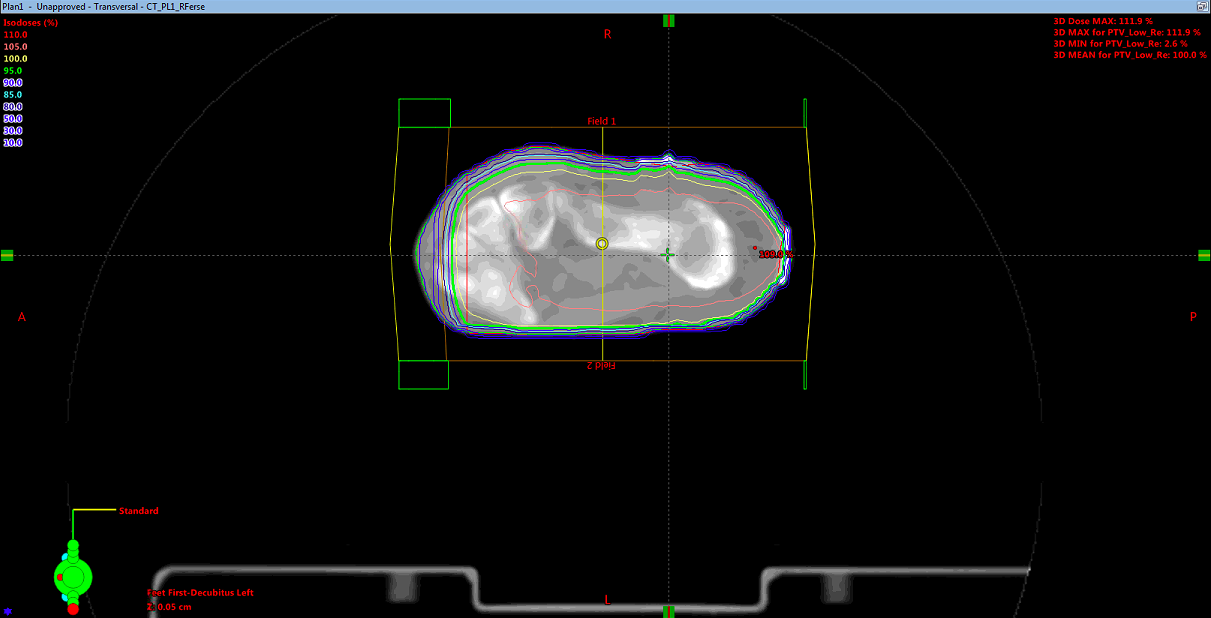
\includegraphics[width=\textwidth]{Bilder/ZAnsicht.png}
  \caption{Darstellung der Dosisverteilung im Fuß in Transversalansicht.}
  \label{abb:z}
\end{figure}

\begin{figure}[H]
  \centering
  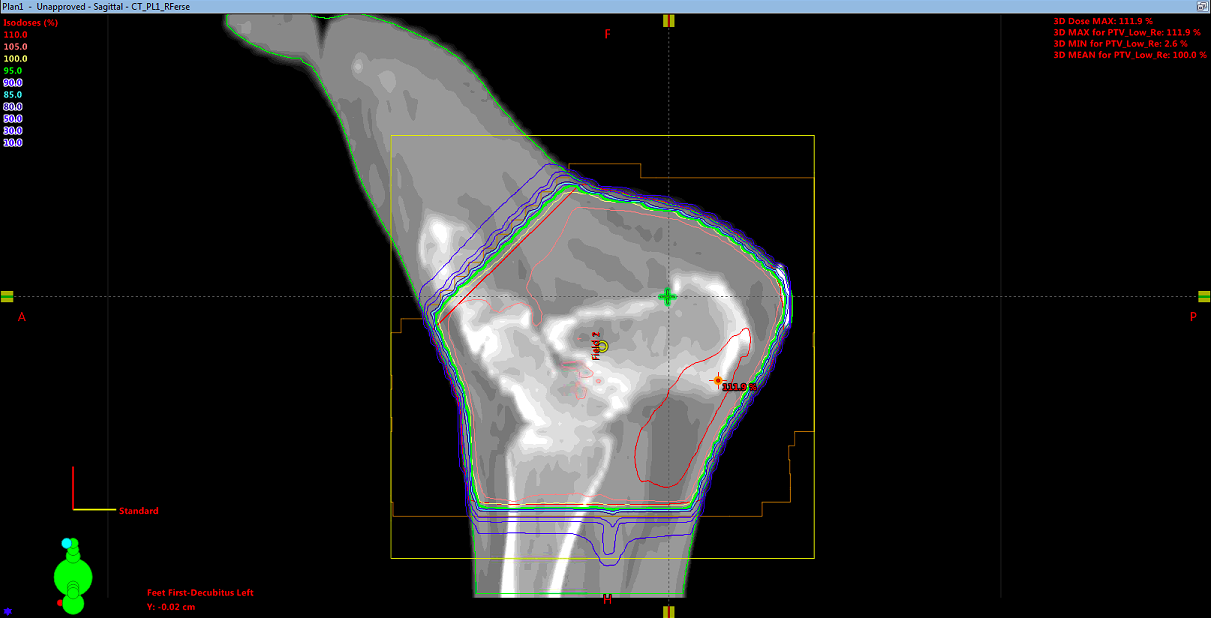
\includegraphics[width=\textwidth]{Bilder/YAnsicht.png}
  \caption{Darstellung der Dosisverteilung im Fuß in Sagittalansicht.}
  \label{abb:y}
\end{figure}

\begin{figure}[H]
  \centering
  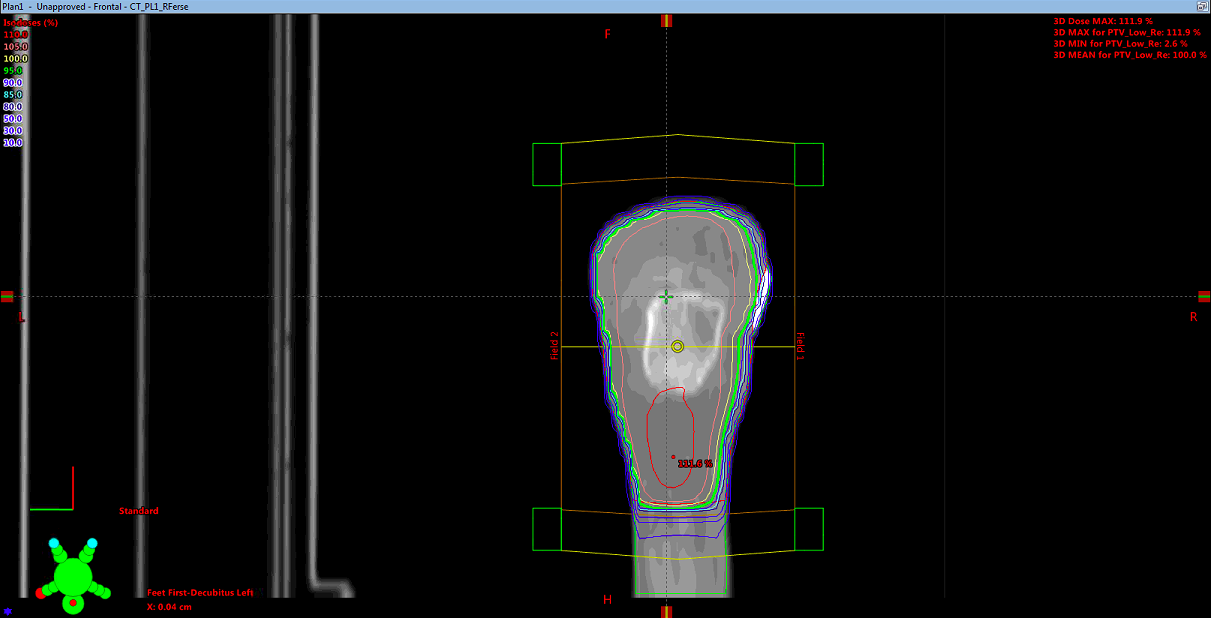
\includegraphics[width=\textwidth]{Bilder/XAnsicht.png}
  \caption{Darstellung der Dosisverteilung im Fuß in Frontalansicht.}
  \label{abb:x}
\end{figure}

In diesen Abbildungen ist das PTV durch eine rote Linie umrandet.
Bei der Erstellung des Bestrahlungsplanes hat sich das Problem ergeben, dass das PTV
bis zur Hautoberfläche eingezeichnet wurde.
Aufgrund des Dosisaufbaueffektes liegt das Dosismaximum bei diesen Photonenenergieen
nicht direkt an der Hautoberfläche, sondern in einer bestimmten Tiefe des Körpers.
Aus diesem Grund ist es nicht möglich an der Hautoberfläche die gewünschte Dosis von
$95\%$ zu erhalten. An diesen Stellen verläuft die $95\%$ Isodosenlinie innerhalb des
Zielvolumens. An den Stellen, wo das Zielvolumen nicht an der Hautoberfläche endet,
liegt die $95\%$ Isodosenlinie außerhalb des Zielvolumens, wie es verlangt wurde. \\

Um die Dosisverteilung in dem PTV und in dem Fuß selber besser beurteilen zu können
ist in Abbildung \ref{abb:DVH} das Dosis-Volumen-Histogramm dargestellt.

\begin{figure}[H]
  \centering
  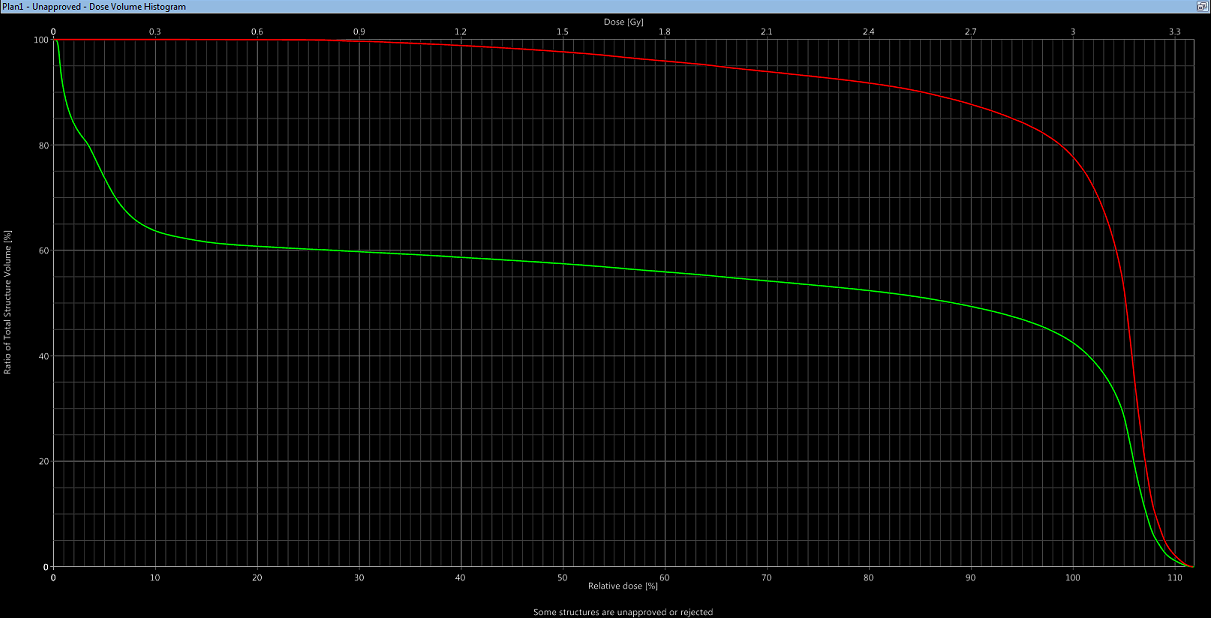
\includegraphics[width=\textwidth]{Bilder/DVH.png}
  \caption{Dosis-Volumen-Histogramm für das PTV in rot und dem gesamten Fuß in grün.}
  \label{abb:DVH}
\end{figure}

Das Ziel, dass das gesamte PTV $95\%$ der applizierten Dosis erhält konnte nicht erreicht werden.
Anhand des DVHs ist zu erkennen, dass etwa $85\%$ des Planungszielvolumens mehr als $95\%$ der applizierten Dosis erhält.
Das liegt daran, dass nicht das gesamte PTV von der $95\%$ Isodosenlinie umgeschlossen werden konnte aus den erläuterten Gründen.
Außerdem beträgt die maximale relative Dosis im PTV $111,9 \%$. Diese maximale Dosis ist um $4,9\%$ größer
als die in der ICRU vorgeschriebene maximale Isodose von $107 \%$ \cite{ICRU}. An dem
DVH ist zu erkennen, dass nur ein sehr geringer Anteil des PTVs diese Dosis erhält.
Außerdem wird diese hohe Dosis nur in dem Zielvolumen deponiert, was anhand der
Dargestellten Dosisverteilungen in den Abbildungen \ref{abb:z}, \ref{abb:y}, \ref{abb:x} gesehen werden kann. \\

Anhand des DVHs für die Body-Kontur ist zu erkennen, dass etwa $57\%$ des gesamten Fußes noch eine
relative Dosis von $50\%$ erhält und über $40\%$ $100\%$ der applizierten Dosis erhält.
Da sich in der Umgebung des PTVs keine Risikoorgane befinden und es sich bei dieser
Therapie um relativ geringe Fraktionsdosen handelt ist es akzeptabel, dass
ein Teil Body-Kontur eine hohe relative Dosis erhält. \\

Dadurch, dass für diese Bestrahlung zwei Felder verwendet worden sind, kann
weitgehend gewährleistet werden, dass das PTV die gewünschte relative Dosis erhält.
Durch die MLCs, die an die Form des Fußes angepasst worden sind, wird das gesunde
Gewebe etwas geschont.
Es hätte durch weitere Felder und genauere Einstellung der MLCs eventuell eine bessere Dosisverteilung erreicht
werden können. Das wäre in diesem Fall allerdings nicht Sinnvoll, da es nur
begrenzt gut möglich ist den Fuß exakt zu positionieren.
